

\documentclass[../../main.tex]{subfiles}


\begin{document}

\section{Introducci\'on}
Se construyo dos circuitos con Amplificadores operacionales. El primero es un circuito inversor, cuya salida es opuesta a la entrada y se la aplifica o atenua, de a cuerdo a como se lo configure. El segundo es no inversor, igual que el primero, atenua o amplifica la señal de entrada, pero no la invierte.
El objetivo es comparar tres modelos del Amplificador Operacional, el modelo ideal, con Avol finito y con Avol dependiendo de la frecuencia. Para ello se comparo la respuesta en frecuencia de los ciruitos mensionados, con la respuesta en frecuencia simulada en LTspice y la simulacion matematica en Matlab.


\section{An\'alisis de los circuitos}

\subsection{Circuito A}

\begin{figure}[H]
\centering

\begin{circuitikz}[scale=1]
\def\xspacing{2}
\def\xstart{0}
\def\yspacing{2}	
\def\ystart{0}

%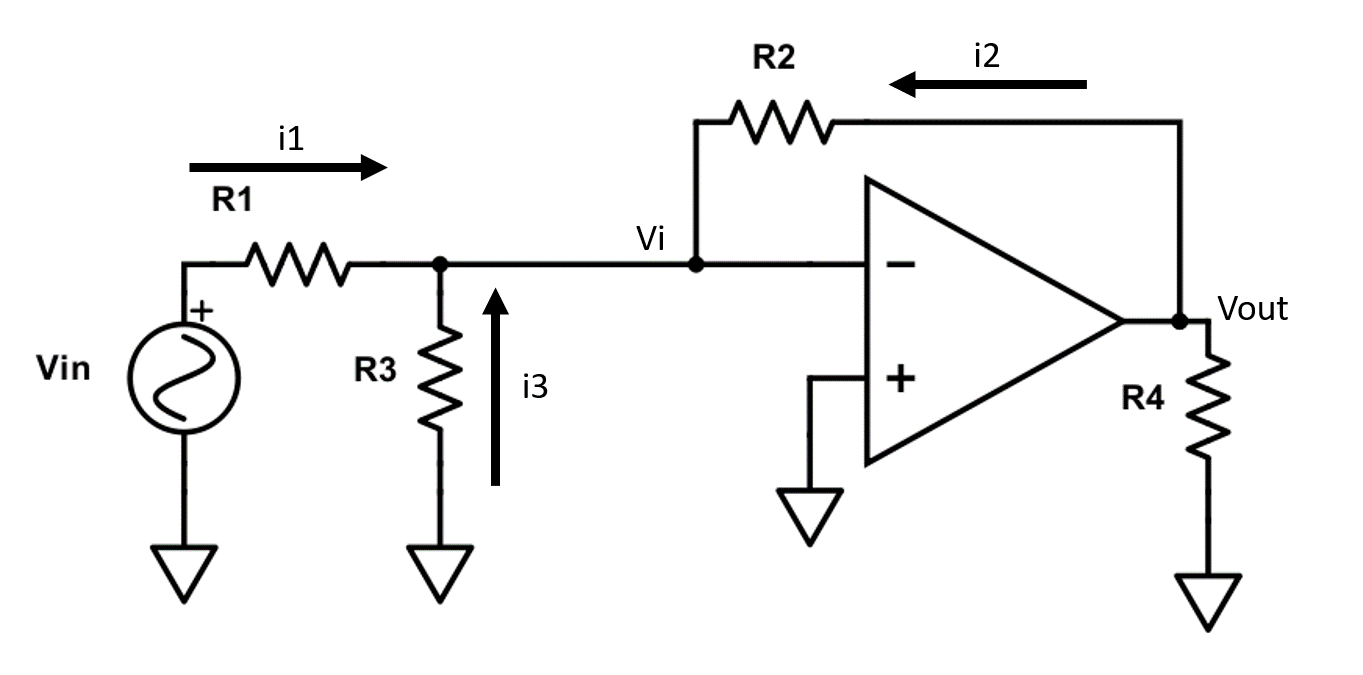
\includegraphics[width=0.5\textwidth]{imagenes/xxx.png}




%dibujo malla izquierda
\draw   						(\xstart, \ystart) node[ground]{}
		to [vsourcesin]	 	(\xstart, \ystart + \yspacing)
		to [R=$R_1$, i>^=$i_1$] (\xstart + \xspacing, \ystart + \yspacing)
		to [R=$R_3$, i<^=$i_3$] (\xstart + \xspacing, \ystart)
		to (\xstart + \xspacing, \ystart) node[ground]{}

%dibujo opamp
%el opamp tiene la misma altura que scale, y las patitas - y + estan en .25*scale y .75*scale
%nos queda - en ystart+yspacing y + en ystart+spacing-0.5

		(\xstart + 3*\xspacing, \ystart + \yspacing - .5) node[op amp] (opamp) {}

%dibujo conexiones a opamp
	 						   (\xstart + \xspacing, \ystart + \yspacing)
		to [short]			  (opamp.-)
								(opamp.+)
		to [short]			  ($(opamp.+)+(0,-\yspacing + 1)$) node[ground]{}	%se me va la patita
								(\xstart + 2*\xspacing, \ystart + 1*\yspacing)
		to [short, *-]		  (\xstart + 2*\xspacing, \ystart + 1.7*\yspacing)
		to [R=$R_2$, i<^=$i_2$] (\xstart + 4*\xspacing, \ystart + 1.7*\yspacing)
		to [short, -*]		  (\xstart + 4*\xspacing, \ystart + 1*\yspacing -.5)
		to [short]			  (opamp.out)
								(\xstart + 4*\xspacing, \ystart + 1*\yspacing -.5)
		to [R=$R_4$]			(\xstart + 4*\xspacing, \ystart) node[ground]{};


\end{circuitikz}


\caption{Esquematico del circuito A}
\end{figure}


\subsubsection{Caso $A_{vol}$ infinito}

Como $A_{vol}$ lo consideramos infinito entonces $V_{i}=0$ \big( tierra virtual \big).Por ende $i_{3}=0$ y $i_{2}=-i_{1}$.
\begin{gather}
V_{out}=-\frac{i_{1}}{R_{2}}\label{eq=CircuitoA6}\\
i_{1}=\frac{V_{in}}{R_{1}}\label{eq=CircuitoA7}
\end{gather}
Reemplazando \ref{eq=CircuitoA7} en \ref{eq=CircuitoA6} y operando algebraicamente se obtine:
\begin{equation}
\frac{V_{out}}{V_{in}}= -\frac{R_{2}}{R_{1}} \label{eq=CircuitoAideal}
\end{equation}


\subsubsection{Caso $A_{vol}$ finito}


\begin{gather}
V_{out}= -V_{i}\cdot A_{vol}\label{eq=CircuitoA1}\\
i_{1}=\frac{V_{in}-V{i}}{R_{1}}\label{eq=CircuitoA2}\\
i_{2}=\frac{V_{out}-V_{i}}{R_{2}}\label{eq=CircuitoA3}\\
i_{3}=\frac{-V_{i}}{R_{3}}\label{eq=CircuitoA4}\\
i_{1}+i_{2}+i_{3}=0\label{eq=CircuitoA5}
\end{gather}

Reemplazando \ref{eq=CircuitoA1},\ref{eq=CircuitoA2},\ref{eq=CircuitoA3},\ref{eq=CircuitoA4} en \ref{eq=CircuitoA5}, se obtiene:


$$\frac{V_{in}}{R_{1}} + \frac{V_{out}}{R_{2}}+\frac{V_{out}}{A_{vol}}\cdot \bigg( \frac{1}{R_{1}} + \frac{1}{R_{2}} + \frac{1}{R_{3}} \bigg) = 0$$

Operando algebraicamente, se obtiene:

\begin{equation}
\frac{V_{out}}{V_{in}}= - \frac{A_{vol} \cdot R_{2} \cdot R_{3}}{A_{vol}\cdot R_{1} \cdot R_{3} + R_{2} \cdot R_{3} +  R_{1} \cdot R_{3} + R_{1} \cdot R_{2} }\label{eq=gananciaAfinito}
\end{equation}
Observacion

$$ \lim_{A_{vol}\to\infty} \big( \ref{eq=gananciaAfinito} \big) = -\frac{R_{2}}{R_{1}} $$
La expresion se redujo a la ganancia del circuito, con el apmlificador operacional ideal\\ \big(\ref{eq=CircuitoAideal}\big).

\subsubsection{Caso $A_{vol}$  con polo dominante}

\begin{equation}
A_{vol }=\frac{A}{1+\frac{s}{W_{p}}}\label{eq=AvolWp}\\
\end{equation} 

Reemplazando \big(\ref{eq=AvolWp}\big) en  \big(\ref{eq=gananciaAfinito}\big)  se obtiene:

\begin{equation}
\frac{V_{out}}{V_{in}}= - \frac{\frac{A}{1+\frac{s}{W_{p}}} \cdot R_{2} \cdot R_{3}}{\frac{A}{1+\frac{s}{W_{p}}}\cdot R_{1} \cdot R_{3} + R_{2} \cdot R_{3} +  R_{1} \cdot R_{3} + R_{1} \cdot R_{2} }
\end{equation}





\end{document}
